% !TeX TXS-program:compile = txs:///arara
% arara: lualatex: {shell: no, synctex: yes, interaction: batchmode}
% arara: pythontex: {rerun: modified} if found('pytxcode', 'PYTHONTEX#py')
% arara: lualatex: {shell: no, synctex: yes, interaction: batchmode} if found('pytxcode', 'PYTHONTEX#py')
% arara: lualatex: {shell: no, synctex: yes, interaction: batchmode} if found('log', '(undefined references|Please rerun|Rerun to get)')

\documentclass[a4paper,11pt]{article}
\usepackage[revgoku]{cp-base}
\graphicspath{{./graphics/}}
%variables
\donnees[%
	classe=1\up*{ère} 2M2,
	matiere={[SPÉ.MATHS]},
	typedoc=TD,
	numdoc=08,
	mois=Juin,
	annee=2022
	]

%formatage
\author{Pierquet}
\title{\nomfichier}
\hypersetup{pdfauthor={Pierquet},pdftitle={\nomfichier},allbordercolors=white,pdfborder=0 0 0,pdfstartview=FitH}
%divers
\lhead{\entete{\matiere}}
\chead{\entete{\lycee}}
\rhead{\entete{\classe{} - \mois{} \annee}}
\lfoot{\pied{\matiere}}
\cfoot{\logolycee{}}
\rfoot{\pied{\numeropagetot}}

\begin{document}

\pagestyle{fancy}

\part{TD08 - Fonction exponentielle en situation (Correction)}

\smallskip

\textbf{\large Partie A}
%
\begin{enumerate}
	\item Graphiquement, le \textcolor{purple}{maximum} de la fonction $f$ est estimé à 147 (pour $x=5$).
	\item Graphiquement, les \textcolor{ForestGreen}{solutions} de $f(x)=100$ sont approximativement $1,8$ et $10,8$.
\end{enumerate}

\begin{center}
	\begin{tikzpicture}[x=0.8cm,y=0.08cm,xmin=0,xmax=21,xgrille=1,xgrilles=0.2,ymin=0,ymax=155,ygrille=10,ygrilles=2]
		\tgrilles \tgrillep \axestikz*
		\axextikz[size=\small]{0,1,...,20} \axeytikz[size=\small]{0,10,...,150}
		%\clip (\xmin,\ymin) rectangle (\xmax,\ymax) ;
		\draw[very thick,red,domain=1:20,samples=500] plot (\x,{80*\x*exp(-0.2*\x)}) ;
		\draw[red] (1.5,65) node {\Large $\mathscr{C}_f$} ;
		\draw[very thick,densely dashed,purple] (5,0) |- (0,147.15) ;
		\filldraw[purple] (5,147.15) circle[radius=2.5pt] ;
		\draw[very thick,densely dashed,ForestGreen] (1.79,0) |- (0,100) (10.76,0) |- (0,100) ;
		\filldraw[ForestGreen] (1.79,100) circle[radius=2.5pt] (10.76,100) circle[radius=2.5pt] ;
	\end{tikzpicture}
\end{center}

\textbf{\large Partie B}
%
\begin{enumerate}
	\item
	\begin{enumerate}
		\item La fonction $f$ est dérivable sur $\intervFF{1}{20}$ par produit, avec $\begin{dcases} u=80x \\ v=\e^{-0,2x} \end{dcases}$ et $\begin{dcases} u'=80 \\ v=-0,2\e^{-0,2x} \end{dcases}$.
		
		Ainsi $f'(x)=u'v+v'u=80 \times \e^{-0,2x} + \left(-0,2\e^{-0,2x}\right) \times 80x = 80 \e^{-0,2x} \times (1-0,2x)$.
		\item $f'(x)$ se présente comme un produit, avec déjà $80\e^{-0,2x} > 0$, et $1-0,2x=0 \ssi 0,2x=1 \ssi x=5$.
		
		\begin{center}
			\begin{tikzpicture}
				\tkzTabInit{$x$/1,$80\e^{-0,2x}$/1,$(1-{0,2}x)$/1,$f'(x)$/1}{$1$,$5$,$20$}
				\tkzTabLine{,+,t,+,}
				\tkzTabLine{,+,z,-,}
				\tkzTabLine{,+,z,-,}
				\aidesignetkztabPL[code=da-,racines={5},couleur=orange]{2}
			\end{tikzpicture}
		\end{center}
		\pagebreak
		\item On en déduit le tableau de variations de la fonction $f$ (les images étant arrondies au centième) :
		
		\begin{center}
			\begin{tikzpicture}
				\tkzTabInit[deltacl=0.8]{$x$/1,$f'(x)$/1,$f$/2}{$1$,$5$,$20$}
				\tkzTabLine{,+,z,-,}
				\tkzTabVar{-/${65,50}$,+/${147,15}$,-/${29,31}$}
				\tkzTabVal[draw]{1}{2}{0.55}{\small \red $\alpha$}{\small \red 100}
				\tkzTabVal[draw]{2}{3}{0.55}{\small \red $\beta$}{\small \red 100}
			\end{tikzpicture}
		\end{center}
	\end{enumerate}
	\item D'après le tableau de variations, $f$ est croissante sur $\intervFF{1}{5}$ et $\begin{dcases} f(1) < 100 \\ f(5) > 100 \end{dcases}$.
	
	L'équation $f(x)=100$ admet de ce fait une unique solution ($\alpha$) sur $\intervFF{1}{5}$.
	
	D'après la fonction TABLE de la calculatrice, $\left. \begin{dcases} f(1,78) \approx 99,474 \\ f(1,79) \approx 100,11 \end{dcases} \right| \Rightarrow \alpha \approx 1,79$.
\end{enumerate}

\begin{pointcalc}
	\hfill\includegraphics[height=3cm]{td08_corr_a}~~~\includegraphics[height=3cm]{td08_corr_b}~~~\includegraphics[height=3cm]{td08_corr_c}\hfill~
\end{pointcalc}

\textbf{\large Partie C}
%
\begin{enumerate}
	\item D'après la question \textbf{A.}\ptno{1} ou la question \textbf{B.}\ptno{1}\pta{c}, on peut affirmer que la bénéfice maximal réalisé par la start-up est de \num{14715}\,€ ($147,15$ centaines) pour 500 (5 centaines) d'ordinateurs fabriqués.
	\item D'après la question \textbf{A.}\ptno{2} ou la question \textbf{B.}\ptno{2}, pour que la start-up réalise un bénéfice supérieur ou égal à 10\,000\,€, elle doit fabriquer entre 179 et 1\,076 ($\alpha$ et $\beta$ centaines) ordinateurs.
\end{enumerate}

\end{document}